%%%% CS553 Cryptography Term Paper TEMPLATE %%%%

%%%% 1. DOCUMENTCLASS %%%%
\documentclass[preprint]{transcrypto}
%%%% NOTES:
% - Change "submission" to "final" for final version
% - Add "spthm" for LNCS-like theorems


%%%% 2. PACKAGES %%%%
\usepackage{lipsum} % Example package -- can be removed
\usepackage{subcaption}
\usepackage{url}
%%%% 3. AUTHOR, INSTITUTE %%%%
\author{Swapnil Narad \\ Devansh Chaudhary \\ Aditya Susawat }
\institute{
  IIT Bhilai, Raipur, India, \email{swapniln@iitbhilai.ac.in}
  \and
  IIT Bhilai, Raipur, India, \email{devanshc@iitbhilai.ac.in}
  \and
  IIT Bhilai, Raipur, India, \email{adityaks@iitbhilai.ac.in}
}
%%%% 4. TITLE %%%%
\title{Khazad-Block-Cipher}
%%%% NOTES:
% - If the title is too long, or includes special macro, please
%   provide a "running title" as optional argument: \title[Short]{Long}
% - You can provide an optional subtitle with \subtitle.

\begin{document}

\maketitle


%%%% 5. KEYWORDS %%%%
\keywords{encryption, decryption, integral, differential}


%%%% 6. ABSTRACT %%%%
\begin{abstract}
   This paper contains a detailed report on the KHAZAD cipher. This paper gives a brief history of the KHAZAD cipher followed by some features of the cipher like block size, key size, etc. The implementation of the KHAZAD cipher is also mentioned in this paper and it contains a detailed description of the key expansion algorithm, general round structure of the cipher, the encryption algorithm, the decryption algorithm, and the code in python for the cipher implementation. This paper also has details about the s-box of KHAZAD and various attacks on the cipher like differential attack, integral attack, etc. on a round reduced variant of the KHAZAD cipher. Finally, it also contains the details about the security and key features of the cipher and the brownie point for our work done. \\
\end{abstract}


%%%% 7. PAPER CONTENT %%%%
\section{Introduction}
KHAZAD is a symmetrical block cipher developed by two cryptographers: Belgian Vincent Reimen (author of the cipher Rijndael) and Brazilian Paulo Barreto. \cite{4}\\
KHAZAD was presented at the European competition of cryptographic primitives NESSIE in 2000.\\
\textbf{Key Size}: 128 bits\\
\textbf{Block Size}: 64 bit (8 bytes) \\

The predecessor of the KHAZAD algorithm is considered to be the SHARK code developed in 1995 by Vincent Rayman and Joan Dimen. The authors of KHAZAD claim that the algorithm is based on the strategy of developing cryptographically stable encryption algorithms (Wide-Trail strategy), proposed by Joan Dimen.\\

The KHAZAD algorithm has conservative parameters and is designed to replace existing ciphers with a 64-bit block, such as IDEA and DES, providing a higher level of security at high execution speeds.\\

Involution transformations are widely used in ciphers, which minimizes the difference between encryption and decryption algorithms.\\ \cite{3}
\begin{center}
        \begin{table}[h]
\begin{tabular}{|c|c|}
\hline
\textit{Name}                                        & \textbf{KHAZAD}                                      \\ \hline
\textit{Number of rounds}                            & \textbf{8}                                           \\ \hline
\textit{Schedule (extension) of the key}             & \textbf{The Feistel scheme}                          \\ \hline
\textit{Unreduced polynomial of the field GF$(2^8)$} & \textbf{$x^8 + x^4 + x^3 + x^2 + 1$}                 \\ \hline
\textit{Implementation of the S-box}                 & \textbf{Recursive P - and Q-miniblocks} \\ \hline
\textit{Implementation of the mixing matrix}         & \textbf{Involutional MDS code}                       \\ \hline
\end{tabular}
\end{table}
\end{center}
\newpage
\section{Main Result}
\label{sec:main}

\subsection{Brief Description}
It's an block cipher that has a single variant block size of 64 bits with a key of single variant of size 128 bits. The input data block is served as a string of 8 bytes.
\\ \\ 
The S-box and the mixing matrix are chosen in a way which ensures that the process of encryption and decryption are the same, except the round connections.
\\ \\
KHAZAD, like the AES algorithm (Rijndael), is from a family of block ciphers which are formed from the SHARK cipher.
\begin{center}
    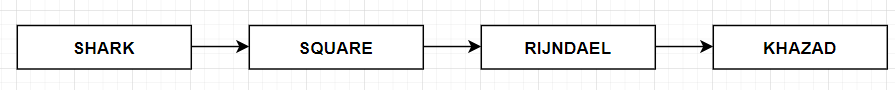
\includegraphics[scale=0.5]{Screenshots/BLOCK1.png}
\end{center}
\subsection{The Implementation Algorithm : }
\begin{itemize}
    \item  Apply key extension algorithm to the key results in a set of round keys.
    \item The algorithm have 8 rounds, each of which consists of 3 stages:
    \begin{enumerate}
        \item \textit{Nonlinear Transformation $\gamma$} 
        \item \textit{Linear Transformation $\theta$ }
        \item \textit{Adding a round key $\sigma$}
    \end{enumerate}
    \item Set of round keys  $k_{0} \ . . . \ k_{8}$ obtained by applying to the encryption key K key extension procedures.
    \item Before the first round $\sigma(k_0)$ is performed.
    \item Operation $\theta$  is not performed in the last round.
\end{itemize} 
\subsection{Key Expansion}
\begin{itemize}
    \item 128-bit (16-byte) key K is divided into 2 equal parts:
    \item $k_{-1}$ - older 8 bytes (from the 15th to the 8th) 
    \item $k_{-2}$ - lower 8 bytes (from the 7th to the 0th) 
    \item Keys $k_{0} \ .\ .\ . \ k_{8}$ calculated according to the Feistel scheme : 
    \item $k_{i} = f(C_{i}, k_{i-1}) \oplus k_{i-2}$ 
\end{itemize}
Here:\\ \\
$f(x, y)$ - round function of the algorithm with the input block x and the key y.\\ \\
$C_{i}$ - 64-bit constant, j which byte is $C_{i}^{j} = S (8i + j)$ \\ \\
\begin{center}
    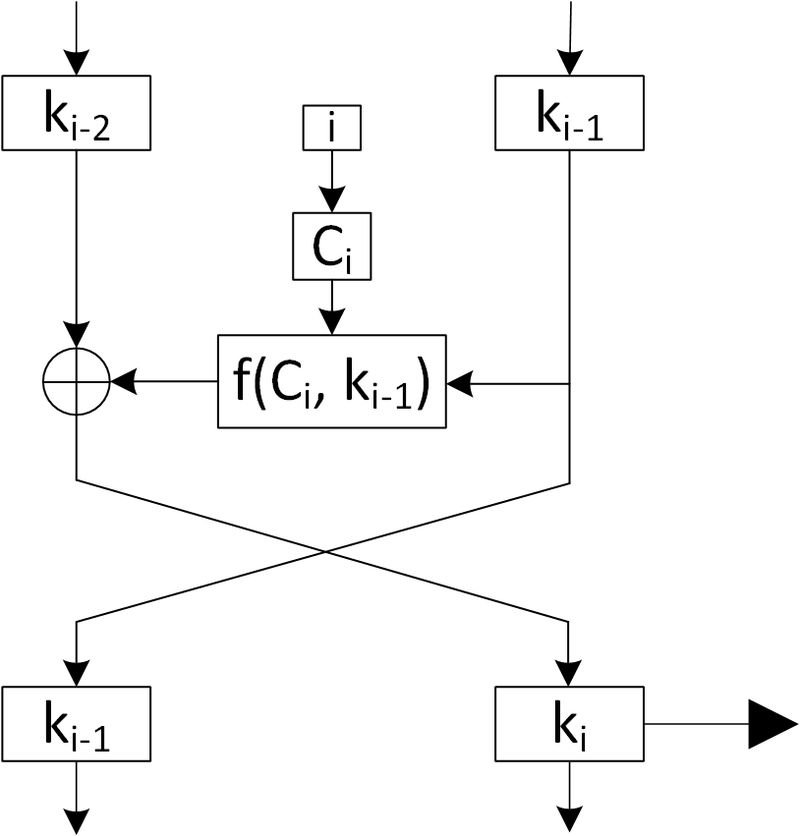
\includegraphics[scale=0.2]{Screenshots/KHAZAD_Key_Schedule_Feistel.jpg}
\end{center}
\subsection{General Round Structure}


    \subsubsection{Nonlinear transformation}
    Denoted as $\gamma$. In each round, the input block is divided into smaller blocks of 8 bytes, which are independently subjected to nonlinear transformation (change), i.e. pass in parallel through the same S-blocks (each S-block - 8x8 bits, i.e. 8 bits at the input and 8 bits at the output).\\ \\
    Replacement blocks in the source and modified (tweaked) ciphers are different. The substitution unit is selected so that the nonlinear transformation is involutionary, i.e. $\gamma = \gamma^{-1} \ or \ \gamma(\gamma(x)) = x.$
    
    
    \subsubsection{Linear transformation }
    Denoted by $\theta$. An 8-byte row of data is multiplied byte by byte to a fixed matrix H size 8 x 8, and byte multiplication is performed in the Galois field $GF(2^{8})$ with a polynomial that is not given $x^{8} + x^{4} + x^{3} + x^{2} +1 \ (0x11D)$.\cite{2}\\
    \begin{center}
            $\theta (x) = x \times H$ \ where\\ 
            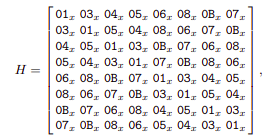
\includegraphics[scale=0.5]{Screenshots/hbox.png}
    \end{center}
    
    
    \subsubsection{Adding a round key }
    A 64-bit XOR operation is performed on the 64-bit data block \& the 64-bit round key .
    A 64-bit data block is been xored with a round key of 64 bits calculated using key expansion algorithm based on Fiestal scheme.\\
   \begin{center}
       For $i^{th} \ round \ : \ \sigma (x_i) = x_{i-1} \oplus k_{i-1}$
   \end{center} 
\subsection{The Encryption and Decryption Algorithm}
\subsubsection{Encryption Algorithm}
    The encryption algorithm is explained below with the help of figure, the figure give good overview of how different layers have been working in course of 8 rounds. \\
    \begin{center}
        \textbf{$ \alpha_{8}[K^0, \ \dots \ K^8] = \sigma[K^8].\gamma.\left(Round_{1}^{7}\right).\sigma[K^0])$}
    \end{center}
\begin{center}
        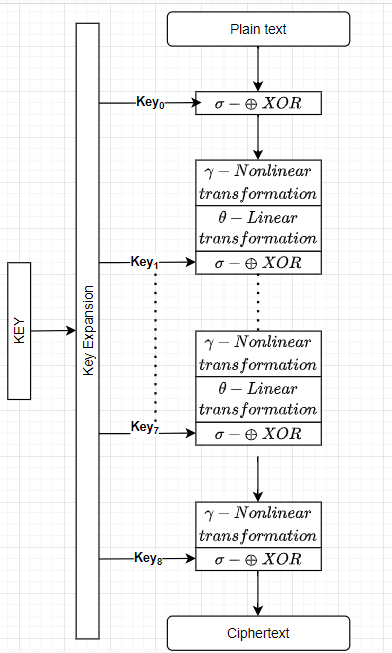
\includegraphics[scale=1]{Screenshots/encrypt.png}\\ 
        \textbf{The Encryption Algorithm}
\end{center} \newpage
\subsubsection{Decryption Algorithm}
The decryption algorithm is explained below with the help of figure, the figure give good overview of how different layers have been working in course of 8 rounds.  \\
\begin{center}
    \textbf{$ \alpha_{8}[K^8, \ \dots \ K^0] = \sigma[K^0].\gamma.\left(Round_{7}^{1}\right).\sigma[K^8])$}
\end{center}
\begin{center}
    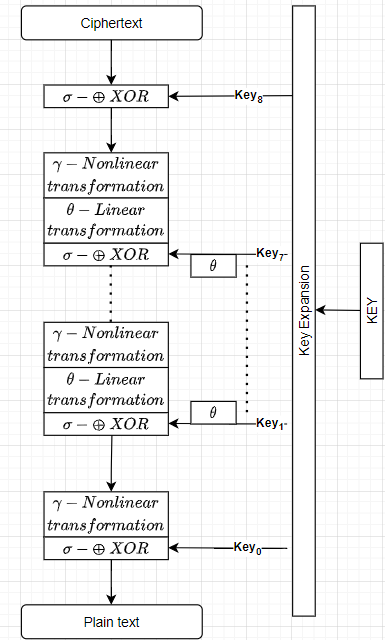
\includegraphics[scale=1]{Screenshots/decrypt.png} \\ 
        \textbf{The Decryption Algorithm}
\end{center}
\newpage
\subsection{The Creation of S-box} 
In the original version of the cipher (KHAZAD-0) tabular replacement was represented by a classic S-block.\\
The bool type definition $GF(2)^{n}\ \longrightarrow$  GF(2) is called Zhegalkin polynomial. The nonlinear order function f is called the order of Zhegalkin's polynomial, i.e. the maximum of the orders of its members.\\
The KHAZAD-0 cipher uses a pseudo random generated S-block that meets the following requirements :
\begin{itemize}
    \item must be an involution
    \item $\delta$-value might not be over $8 \times 2^{-8}$
    \item $\lambda$-value might not be over $16 \times 2^{-16}$
    \item nonlinear order $\nu$ should be a maximum, namely equal to 7
\end{itemize}
In the modified version of the cipher, the S-block 8x8 is modified and represented by a recursive structure consisting of mini-blocks P and Q, each of which is a small replacement block with 4 bits at the input and output (4x4). \\
Recursive structure of the replacement unit in the modified KHAZAD cipher:\cite{2} \\
\begin{center}
    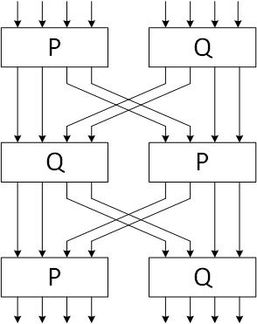
\includegraphics[scale=0.6]{Screenshots/RecStructure.jpg}
\end{center} 
This structure of P - and Q-miniblocks is equivalent to the S-block with the following substitution table:
\begin{center}
    \textbf{Correspondence of output values to inputs for mini-block P \cite{3}} \linebreak
    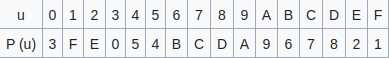
\includegraphics[scale=0.5]{Screenshots/ps1.png}
\end{center}
\begin{center}
    \textbf{Correspondence of output values to inputs for mini-block Q \cite{3}} \linebreak
    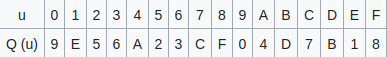
\includegraphics[scale=0.5]{Screenshots/qs1.png}
\end{center}
\newpage
\begin{center}
        \textbf{The final KHAZAD S-box \cite{2}}
        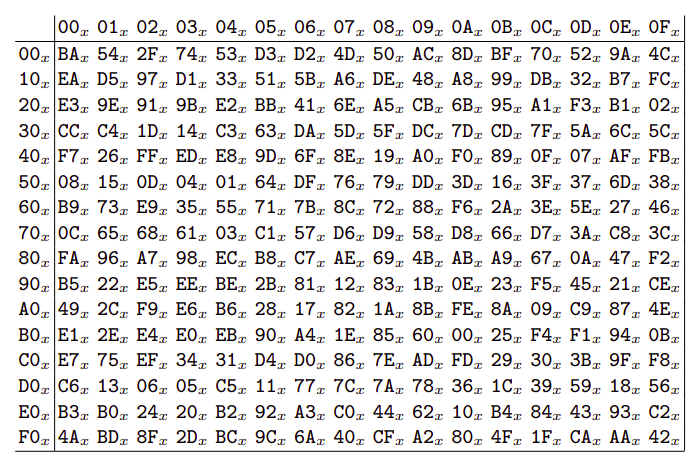
\includegraphics[scale=0.5]{Screenshots/sbox.png}
\end{center}
\subsection{Code Implementation} 
The code file for implementation is provided in the same \textit{github} repository, the test vectors are also provided for the same.
\begin{figure}[H]
		\begin{subfigure}{.5\textwidth}
			\centering
			% include first image
			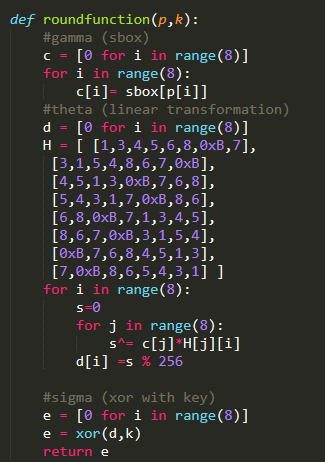
\includegraphics[width=.4\linewidth]{Screenshots/roundr.png}  
			\caption{The code snippet for round structure}
			\label{fig:sub-first}
		\end{subfigure}
		\begin{subfigure}{.5\textwidth}
			\centering
			% include second image
			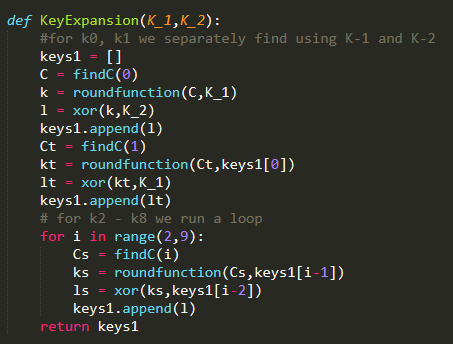
\includegraphics[width=.4\linewidth]{Screenshots/keyex.png}  
			\caption{The code snippet for key expansion algorithm}
			\label{fig:sub-second}
		\end{subfigure}
		\begin{subfigure}{.5\textwidth}
			\centering
			% include second image
			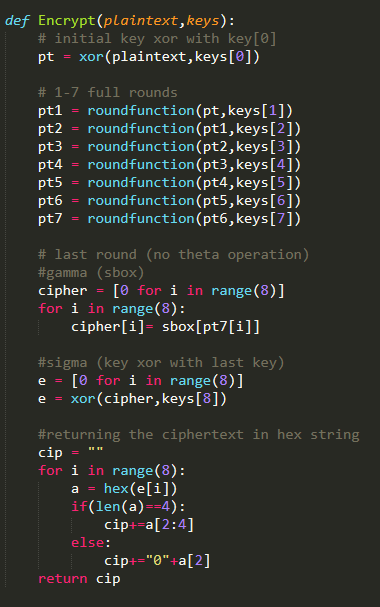
\includegraphics[width=.4\linewidth]{Screenshots/encr.png}  
			\caption{The code snippet for encryption algorithm}
			\label{fig:sub-third}
		\end{subfigure}
		\caption{Implementation code snippets}
		\label{fig:fig:fig}
	\end{figure}
\subsection{Attacks} 
The group of ciphers which include Shark, Square, Rijndael,
Anubis and Khazad are made in such a way that
as far as differential attack and attacks like linear attacks are concerned, it is very unusual
to be successful for these ciphers on their full versions.
\subsubsection{Differential attack}
A differential attack exists for a 3 rounds Khazad cipher but its time complexity is very large as compared to 3 round integral attack which is discussed below. The effect of each round on the message block due to different layers is shown below:\\
\begin{center}
    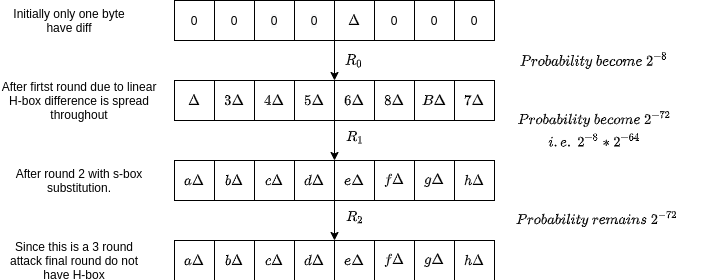
\includegraphics[scale=0.6]{Screenshots/diffat.png} \\
    The attack would follow this strategy:
\end{center}
\begin{center}
    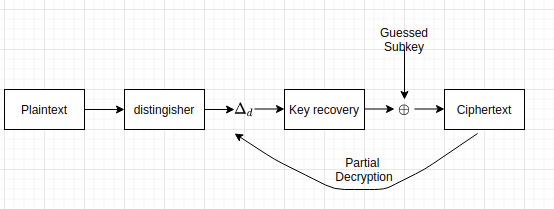
\includegraphics[scale=0.5]{Screenshots/pd.png}
\end{center}
So after guessing 8 bytes of key or guessing subkey there would be at max $2^{64}$ possible guesses for 8 bytes of subkey, therefore the time complexity achieved would be $2^{64}$
\begin{table}[h]
\centering
\begin{tabular}{|l|l|l|}
\hline
Attack Type     & Rounds & Time     \\ \hline
differential attack & 3      & $2^{64}$  \\ \hline
\end{tabular}
\end{table} 
\newpage
\subsubsection{DDT}
The DDT for s-box of KHAZAD can be created similar to how it was created for other block ciphers.
\begin{center}
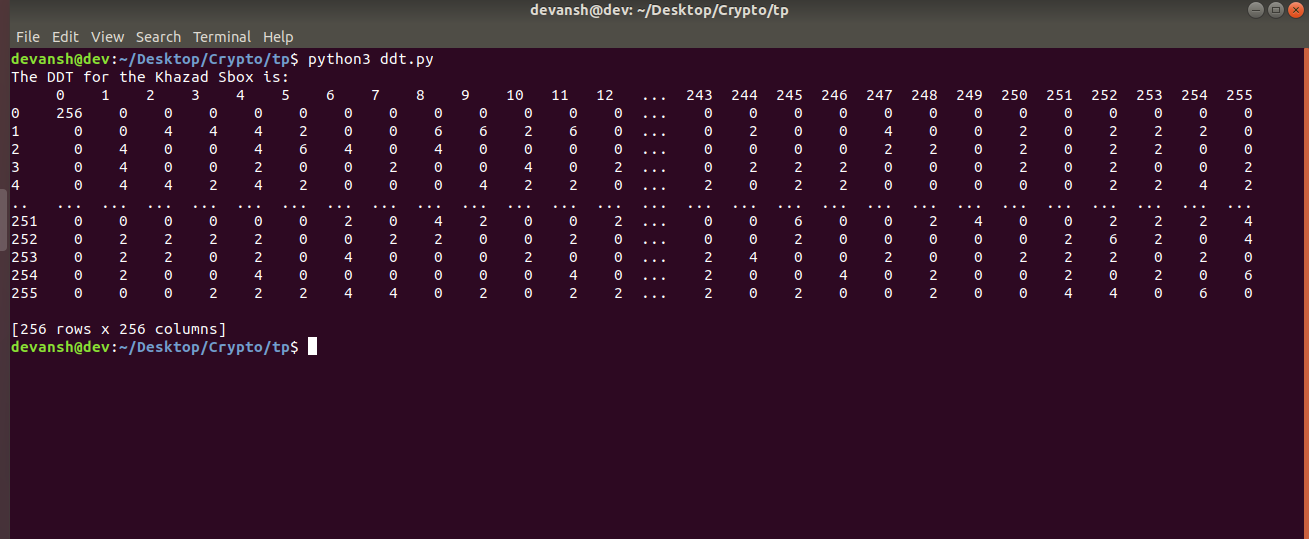
\includegraphics[scale=0.34]{Screenshots/k_ddt1.png}  \\
The horizontal view
\end{center}
\begin{center}
    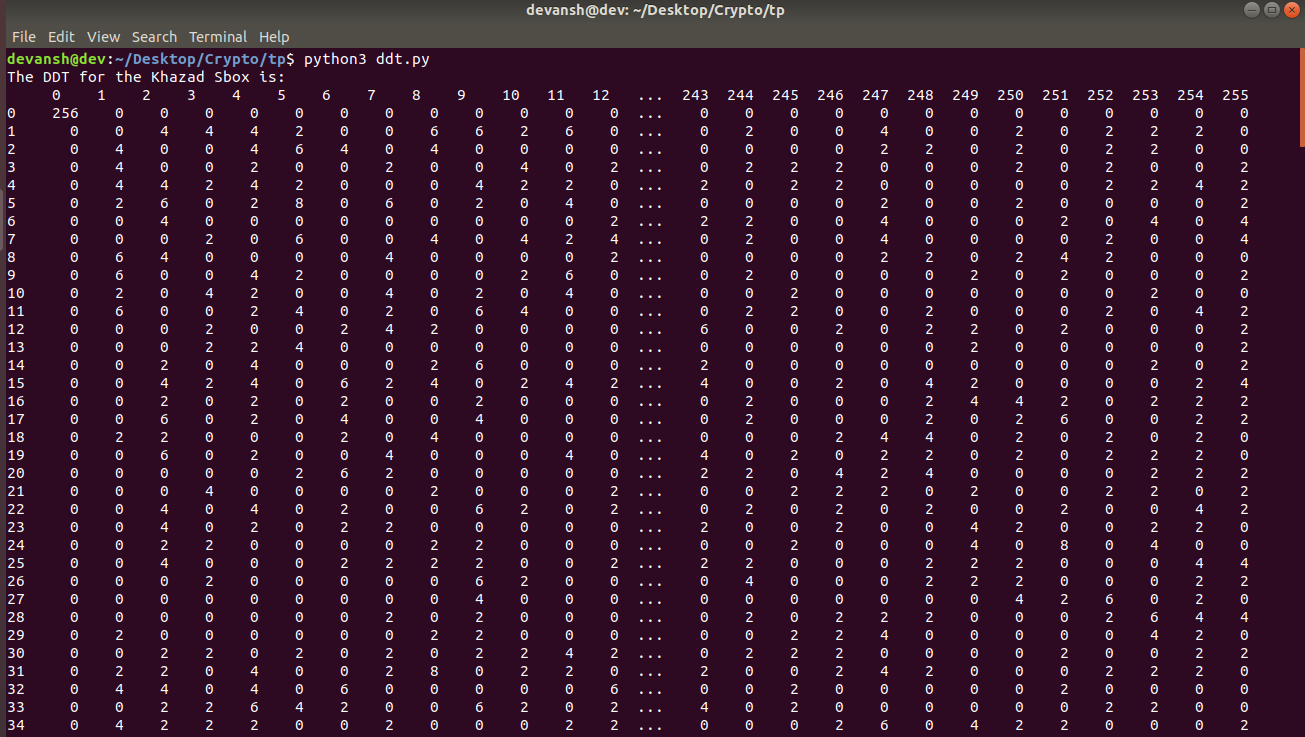
\includegraphics[scale=0.34]{Screenshots/k_ddt.png}\\
    The center view
\end{center}
There were around 100 s-box transitions like 5 -> 5 ,  4 -> 2E,  7 -> 86  having the best probability equal to $\frac{8}{16} = 0.5$. Any of the byte can be taken accordingly for differential attack.
\newpage
\subsubsection{The Integral attack}
Also known as the \textbf{The Square Attack}. The integral attack consists of the following properties.
The attack is set on a
256 plaintexts, such that the first byte takes all 256 possible values
while other bytes have constant values.
\begin{itemize}
    \item \textbf{The All property : }The All property is the byte in which all values come once among the texts in the set. It is denoted by \textit{\textbf{A}}.
    \item \textbf{The Constant property : }The constant property refers to the byte in which all texts in the set have the same value. It is denoted by \textit{\textbf{C}}.
    \item \textbf{The Balanced property : }Also called the 0-sum property, the balanced property refers to the byte in which sum of all the texts in the set is ZERO. It is denoted by \textit{\textbf{B}}.
\end{itemize}
The integral attack on Khazad cipher is explained in the below figure :\cite{1} \\
\begin{center}
    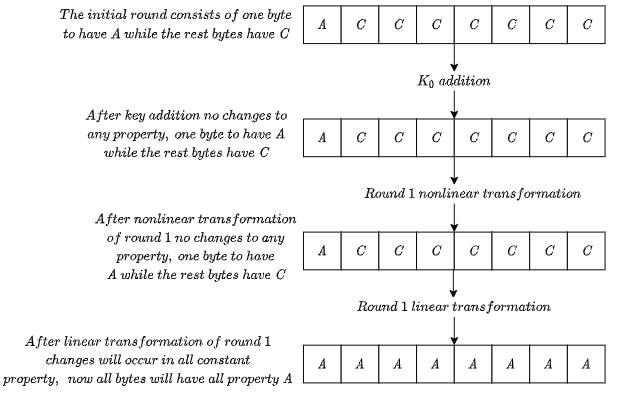
\includegraphics[scale=0.7]{Screenshots/r01.png}  
\end{center} \newpage
\begin{center}
    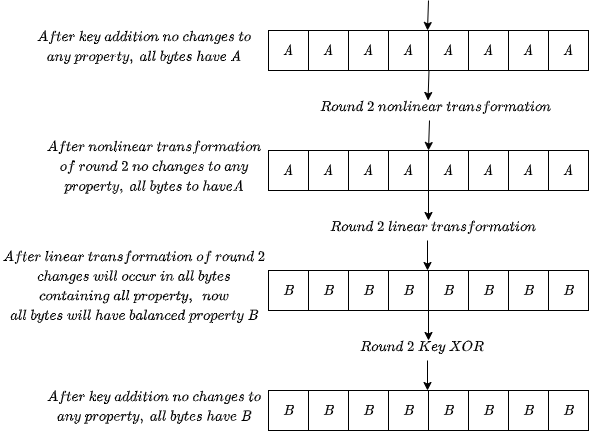
\includegraphics[scale=0.7]{Screenshots/r12.png}  
\end{center} 
So we can say that all bytes in our plaintexts will have balanced property after 2 rounds. Considering the fact that there will be no H-box or linear transformation in the last round, the corresponding subkey bytes can be guessed separately to do a complete 3-rounds attack here.\\
The complexity of this attack will be nearly $2^{16}$ sbox looks and $2^9$ plaintexts selections. Also we can increase this attack to 4 rounds by guessing the other subkey and this will increase time complexity by $2^{64}$.\\
So far we have seen two variants of integral attacks on Khazad in which one is 3 round integral attack where complexity is : \\
\begin{table}[h]
\centering
\begin{tabular}{|l|l|l|l|}
\hline
Attack Type     & Rounds & Time     & Space \\ \hline
integral attack-1 & 3      & $2^{16}$ & $2^9$ \\ \hline
\end{tabular}
\end{table}
\\
The second one is 4 round integral attack where we guess the other subkey.
\begin{table}[h]
\centering
\begin{tabular}{|l|l|l|l|}
\hline
Attack Type     & Rounds & Time     & Space \\ \hline
integral attack-2 & 4      & $2^{80}$ & $2^9$ \\ \hline
\end{tabular}
\end{table}


\newpage

\subsection{Other Attacks}
\subsubsection{Improved Integral attack}\cite{2}
The improved integral attack is basically an extension of integral attack up to 5 rounds and is having following time complexity.\cite{1}
\begin{table}[h]
\centering
\begin{tabular}{|l|l|l|l|}
\hline
Attack Type     & Rounds & Time     & Space \\ \hline
integral attack-3(improved) & 5      & $2^{91}$ & $2^{64}$ \\ \hline
\end{tabular}
\end{table}\\
With the use of key-scheduling algorithm and algebraic properties of round structure, this attack was made possible for 5 round KHAZAD in a very impressive time and space complexity. 
\subsubsection{Weak Keys Attack}\cite{2}
There are various new attacks on Khazad one of which is weak keys attack. The one of better cryptanalytic result on 5-rounds Khazad cipher is the of $2^{64}$ weak keys identified where it can be broken with
$2^{43}$ steps of analysis using $2^{38}$ encryption blocks.\\

\begin{table}[h]
\centering
\begin{tabular}{|l|l|l|l|}
\hline
Attack Type     & Rounds & Time     & Space \\ \hline
Weak Keys & 5      & $2^{43}$ & $2^{38}$ \\ \hline
\end{tabular}
\end{table}

\subsubsection{Interpolation attacks}\cite{2}
This attack generally give benefit using the cipher components having simple algebraic structures like the structure of s-box etc.,that can be used as combined to give
polynomial in feasible complexity.The way s-box of KHAZAD is created,and enforcing the effect of the diffusion
layer, makes an attack of this type infeasible.

\subsubsection{The boomerang attack}\cite{2}
The boomerang attack require ciphers whose encryption and decryption efficiency is different; this is not the case for KHAZAD, as it have
involution structure.

\subsection{Security}
KHAZAD's crypto-resistance is equal to a block cipher with the given block and key lengths. \\
The motive of KHAZAD cipher was to achieve a K-secure and Hermetic secrecy.\\\\
Major security highlights of KHAZAD are :
\begin{itemize}
    \item The most effective attack to find the KHAZAD cipher key is a full search.
    \item In KHAZAD, retrieving information about some Plain-Cipher text pairs from any given Plain-Cipher text pair is as efficient as using complete key search to determine the key.
    \item The approximate complexity of the key search by the full search method is directly dependent on the bit length of the key and is equal to $2^{127}$ applications of KHAZAD. \\
    
\end{itemize}
\subsection{Key-Features}
\begin{itemize}
    \item It is observed that KHAZAD is much better than most of the modern available ciphers as far as compatibility is concerned.
    \item It is a very fast cipher and it avoids using excessive storage space for all of its code and tables.
    \item It does not have uncommon and expensive instruction built for a processor. This is the reason it is good for most platforms.
    \item The maths included in the creation algorithm is not complex and easy to understand.
    \item Since the key schedule is similar to the round function, we don't require any extra storage.
\end{itemize}
\subsection{Brownie Point}
\begin{itemize}
    \item We implemented the key expansion algorithm and the code implementation of the cipher in python language which was not found anywhere and was solely done by us.
    \item We created several figures using \url{draw.io} which would be helpful for the people who wants to understand KHAZAD implementation algorithm and basic attacks on it. These figures were not available online and was solely done by us.
\end{itemize} 
%%Add any more observation here.


%%%% 8. BIBLIOGRAPHY %%%%
\bibliographystyle{alpha}
\bibliography{citations}
%%%% NOTES
% - Download abbrev3.bib and crypto.bib from https://cryptobib.di.ens.fr/
% - Use bilbio.bib for additional references not in the cryptobib database.
%   If possible, take them from DBLP.
\end{document}
 